\chapter{Tehnologii Folosite}

Pentru implementarea propriu-zisa a licentei, a fost utilizat un anumit set de tehnologii, care sa ajute la implementarea motorului fizic si a algoritmului genetic de la un nivel cat mai primitiv, de unde sa poate fie modelat orice tip de comportament dorit.

\section{C++}
 
Mediul de lucru este C++17 \footnote{\url{http://www.cplusplus.com/}}sub Visual Studio 2019. C++ a fost ales in principal datorita performantei si a experientei anterioare. Prin intermediul OOP au fost create structuri pentru o implementare cat mai naturala a motorului fizic si a algoritmului genetic. 

\section{OpenGL}
 
Reprezentarea grafica se realizeaza cu ajutorul librariei OpenGL 3.3\footnote{\url{https://www.opengl.org/}}. Motivatia librariei OpenGL a fost atat introducerea ei in Anul 3 cat si permitarea implementarii cat mai primitiva a motorului fizic.

\section{OpenGL Mathematics (GLM)}
 
Fiind un motor fizic, este necesar ca toate calculele matematice sa fie realizate cat mai corect si rapid, astfel libraria GLM \footnote{\url{https://glm.g-truc.net/0.9.9/index.html/}} a fost aleasa pentru viteza si compatibilitatea ei cu OpenGL.

Principalele structuri folosite din GLM au fost:
\begin{itemize}
    \item glm::vec2/glm::vec3/glm::vec4
    \item glm::quat, (glm quaternions). Motivatia quaternionilor in favoarea matricelor de rotatie a fost performanta si evitarea problemelor unghiurilor euler, cum ar fi Gimbal Lock \footnote{\url{https://en.wikipedia.org/wiki/Gimbal_lock/}}
    \item glm::mat3/glm::mat4
\end{itemize}

Librarii alternative au fost: Eigen \footnote{\url{http://eigen.tuxfamily.org/index.php?title=Main_Page}} si CML \footnote{\url{https://github.com/demianmnave/CML/wiki/The-Configurable-Math-Library}}. Fiecare librarie aduce un anumit punct forte, GLM a fost ales pentru compatibilitatea cu OpenGL. Rezultatele exacte sunt urmatoarele:

\begin{center}
    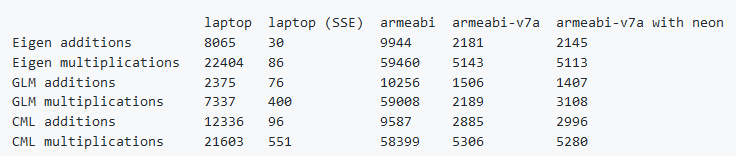
\includegraphics[width=1\textwidth]{math-library-example.png} \textit{source: https://github.com/mfoo/Math-Library-Test} \footnote{\url{https://github.com/mfoo/Math-Library-Test}}
\end{center}




\section{GLFW}
 
Pentru initializarea ferestrei OpenGL a fost folosit GLFW \footnote{\url{https://www.glfw.org/}}. Aceasta librarie ofera in mod simplistic un context OpenGL si mai multe optiuni cum ar fi VSync sau DoubleBuffering. De asemenea,
keyboard si mouse events sunt capturate prin GLFW.

Alternative au fost : GLUT \footnote{\url{http://freeglut.sourceforge.net/}}. GLFW a fost ales in favoarea GLUT deoarece pe masina unde a fost dezvoltata aplicatia, GLUT nu reusea sa intanstieze OpenGL 3.3+.
\section{Concluzii}

C++ impreuna cu OpenGL si GLM ofera un mediu de lucru cat mai aproape de procesor si in acelasi timp un set de structuri si unelte pentru dezvoltarea naturala a Motorului Fizic. Pentru algoritmului genetic, C++ contine deja tot de ce este nevoie si permite implementarea unui algoritm genetic rapid, "from scratch".